\uuid{PA24}
\exo7id{7163}
\auteur{megy}
\organisation{exo7}
\datecreate{2017-06-11}
\isIndication{false}
\isCorrection{true}
\chapitre{Nombres complexes}
\sousChapitre{Géométrie}

\contenu{
\texte{

}
\begin{enumerate}
    \item \question{Soit $ABC$ un triangle. Montrer qu'il est équilatéral direct ssi les affixes (un repère orthonormé direct ayant été fixé) des sommets vérifient $a+bj+cj^2=0$.}
\reponse{Le triangle $ABC$ est équilatéral direct ssi $C$ est l'image de $B$ par la rotation de centre $A$ et d'angle $\pi/3$. Ceci est équivalent à $c-a = e^{i\pi/3}(b-a) = -j^2(b-a)$.
Or, on a :
\begin{align*}
c-a  = -j^2(b-a) 
&\Leftrightarrow c-a(1+j^2)+bj^2=0\\
&\Leftrightarrow aj+bj^2+c=0\\
&\Leftrightarrow  a+bj+cj^2=0.
\end{align*}}
    \item \question{(Notations réinitialisées) Soit $O$ un point du plan,  $\mathcal C$ un cercle de centre $O$, et $A$, $B$, $C$, $D$, $E$ et $F$ des points distincts de $\mathcal C$ vérifiant (dans $\R/2\pi\Z$) l'égalité:
\[ (\overrightarrow{OA},\overrightarrow{OB})
=(\overrightarrow{OC},\overrightarrow{OD})
=(\overrightarrow{OE},\overrightarrow{OF})
=\pi/3.\]

On note $M$ (resp. $N$, $P$) le milieu de $[BC]$ (resp. $[DE]$, $[FA]$). Montrer que $MNP$ est équilatéral direct.}
\reponse{Fixons un repère orthonormé direct de centre $O$. 
\begin{center}
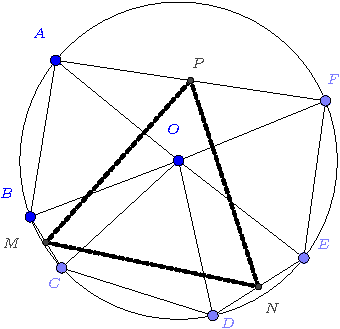
\includegraphics{../images/img007163-1}
\end{center}
D'après l'énoncé, on a $b=-j^2a$, $d=-j^2c$ et $f=-j^2e$. On en déduit:
\begin{align*}
m+jn+j^2p 
&= \frac{b+c+j(d+e)+j^2(f+a)}{2}\\
&=\frac{-j^2a+c+j(-j^2c+e)+j^2(-j^2e+a)}{2}\\
&=\frac{a(j^2-j^2)+c(1-j^3)+e(j-j^4)}{2}\\
&=0.\\
\end{align*}
D'après la première question, $MNP$ est équilatéral direct.}
\end{enumerate}
}
